\chapter{Metodi tradizionali}
La caratteristica degli algoritmi di compressione tradizionali è quella di usare trasformate statiche all’interno del primo blocco, messe a punto in numerosi anni di ricerca. Questa staticità non permette a questi metodi di adattarsi dinamicamente a tutti i tipi di contenuti delle immagini. Inoltre rende lo sviluppo di un nuovo algoritmo di compressione un processo lungo che richiede anni di studi e progettazione. \cite{ cheng2018deep}
Andiamo ora a parlare brevemente dei metodi che andremo a considerare quando valuteremo le prestazioni dei vari algoritmi per poterli confrontare.

\section{JPEG}
Questo metodo di compressione sviluppato nel 1992 è diventato in poco tempo il formato di compressione più diffuso. Nonostante i numerosi tentativi di sostituirlo con formati più moderni questo è rimasto ancora ad oggi il formato più usato, principalmente grazie alla sua facilità implementativa. Il JPEG si basa sull’utilizzo della DCT per realizzare la rappresentazione sparsificata dell’immagine originale. I valori prodotti dall'applicazione della trasformata vengono poi quantizzati e codificati con un metodo denominato zig-zag scan \cite{ 125072} \\
Possiamo vedere un esempio di compressione con JPEG nella figura \ref{fig:CompressionJPEG}

\section{JPEG2000}
Nel 2001 con la crescente diffusione di internet, con l’aumento di dimensione delle immagini e la richiesta di una maggiore qualità da parte degli utenti, viene sviluppato questo nuovo formato chiamato appunto JPEG2000 in virtù dell'anno in cui è stato sviluppato.\\
JPEG2000 non utilizza la DCT come il suo predecessore ma viene introdotta una nuova trasformata, la DWT o Discrete Wavelet Transformat, che si propone di meglio identificare e comprimere i bordi delle figure che compongono le immagini, ovvero il dettaglio che ci permette di distinguere le varie regioni all'interno di un immagine.
JPEG2000 quindi voleva essere un formato di qualità superiore con una compressione più efficiente.\cite{952804}\\
Possiamo vedere un esempio di compressione con JPEG2000 nella figura \ref{fig:CompressionJPEG2000}

\section{BPG}
Questo formato è stato sviluppato da Fabrice Bellard nel 2014 con l'obbiettivo di sostituire l’ormai affermato formato JPEG. Questo metodo di codifica si basa sulla codifica intra-frame del codec HEVC o H.265. \cite{BPGImageformat} Bellard voleva realizzare un formato molto leggero che potesse fornire immagini più compresse rispetto a JPEG, ma con una qualità superiore.\\
Possiamo vedere un esempio di compressione con BPG nella figura \ref{fig:CompressionBPG}

\section{VVC}
Versatile Video Coding (VVC) o H.266 è lo standard di codifica video più recente, finalizzato nel luglio 2020. È stato sviluppato dal Joint Video Experts Team (JVET) dell'ITU-T Video Coding Experts Group (VCEG) e dell'ISO/IEC Moving Picture Experts Group (MPEG) per soddisfare la crescente richiesta di una migliore compressione video e per supportare una più ampia gamma di contenuti multimediali attuali e applicazioni emergenti come contenuti HDR, a 360°, per la Realtà Virtuale (VR) o la Realtà Aumentata (AR).\cite{9503377}\\
Sebbene sia stato sviluppato per la compressione video, fornisce ottimi risultati anche andando a comprimere video contenenti un solo frame, ovvero delle immagini.\\
Possiamo vedere un esempio di compressione con VVC nella figura \ref{fig:CompressionVVC}

\newpage
\begin{figure}
    \centering
    \begin{subfigure}[t]{0.3\textwidth}
        \includegraphics[width=\textwidth]{Immagini/IMAGES/PNG/IMG0004.png}
        \caption{Originale}
        \label{fig:OriginalJPEG}
    \end{subfigure}
    \hspace*{1.5cm}
    \begin{subfigure}[t]{0.3\textwidth}
        \includegraphics[width=\textwidth]{Immagini/IMAGES/JPEG/IMG0004.png}
        \caption{JPEG}
        \label{fig:CompressedJPEG}
    \end{subfigure}
    \caption{Confronto immagini PNG con JPEG bpp medio = 0.174}
    \label{fig:CompressionJPEG}
\end{figure}

\begin{figure}
    \centering
    \begin{subfigure}[t]{0.3\textwidth}
        \includegraphics[width=\textwidth]{Immagini/IMAGES/PNG/IMG0004.png}
        \caption{Originale}
        \label{fig:OriginalJPEG2000}
    \end{subfigure}
    \hspace*{1.5cm}
    \begin{subfigure}[t]{0.3\textwidth}
        \includegraphics[width=\textwidth]{Immagini/IMAGES/JPEG2000/IMG0004.png}
        \caption{JPEG2000}
        \label{fig:CompressedJPEG2000}
    \end{subfigure}
    \caption{Confronto immagini PNG con JPEG2000 bpp medio = 0.171}
    \label{fig:CompressionJPEG2000}
\end{figure}

\begin{figure}
    \centering
    \begin{subfigure}[t]{0.3\textwidth}
        \includegraphics[width=\textwidth]{Immagini/IMAGES/PNG/IMG0004.png}
        \caption{Originale}
        \label{fig:OriginalBPG}
    \end{subfigure}
    \hspace*{1.5cm}
    \begin{subfigure}[t]{0.3\textwidth}
        \includegraphics[width=\textwidth]{Immagini/IMAGES/BPG/IMG0004.png}
        \caption{BPG}
        \label{fig:CompressedBPG}
    \end{subfigure}
    \caption{Confronto immagini PNG con BPG bpp medio = 0.179}
    \label{fig:CompressionBPG}
\end{figure}

\begin{figure}
    \centering
    \begin{subfigure}[t]{0.3\textwidth}
        \includegraphics[width=\textwidth]{Immagini/IMAGES/PNG/IMG0004.png}
        \caption{Originale}
        \label{fig:OriginalVVC}
    \end{subfigure}
    \hspace*{1.5cm}
    \begin{subfigure}[t]{0.3\textwidth}
        \includegraphics[width=\textwidth]{Immagini/IMAGES/VVC/IMG0004.png}
        \caption{VVC}
        \label{fig:CompressedVVC}
    \end{subfigure}
    \caption{Confronto immagini PNG con VVC bpp medio = 0.164}
    \label{fig:CompressionVVC}
\end{figure}